\section{The Desert Camp, Mandawa} % (fold)
\label{sec:dcm}

\subsection{Introduction} % (fold)
\label{sub:dcm_intro}

Four kilometres away from the town of Mandawa in Rajasthan is a cluster of mud huts on a large sand dune. From a distance, they look like any other village homes --- perhaps a shade cleaner and sans the usual clamour of people and their domesticated animals. Upon examining up-close, one realises that these are unique and extraordinary indeed. Designed by the talented Delhi-based architects, Revathi and Vasant Kamath, \emph{The Desert Camp} is quite literally a poem in mud.

It is a project designed to recreate the atmosphere, incorporate images, forms, and spaces of a village in the Shekhawah region of Rajasthan. The facility caters to the middle and upper class international tourists looking for a rural Indian experience. The architecture therefore assumes surrealistic qualities.

% subsection dcm_intro (end)

\subsection{Concept} % (fold)
\label{sub:dcm_concept}

This is a convincing example, proving that it is within the realm of possibility to combine modern creature comforts with basic rural dwellings effectively.

The suites are designed to represent the homes of the village farmer, potter, and weaver, by incorporating the spaces, objects from everyday use, and the relevant tools to craft as practicable an experience as possible.

The architectural farms and elements emerge from the juxtaposition of the requirements of two distinct and divergent lifestyles: meeting the needs and standards of comfort of the western tourist while creating an indigenous and contextual setting for folk artisans and performance at the same time --- as a way to display and market their skills and earn livelihood in an environment that is akin to their own habitat.

\begin{figure}[H]
  \centering
  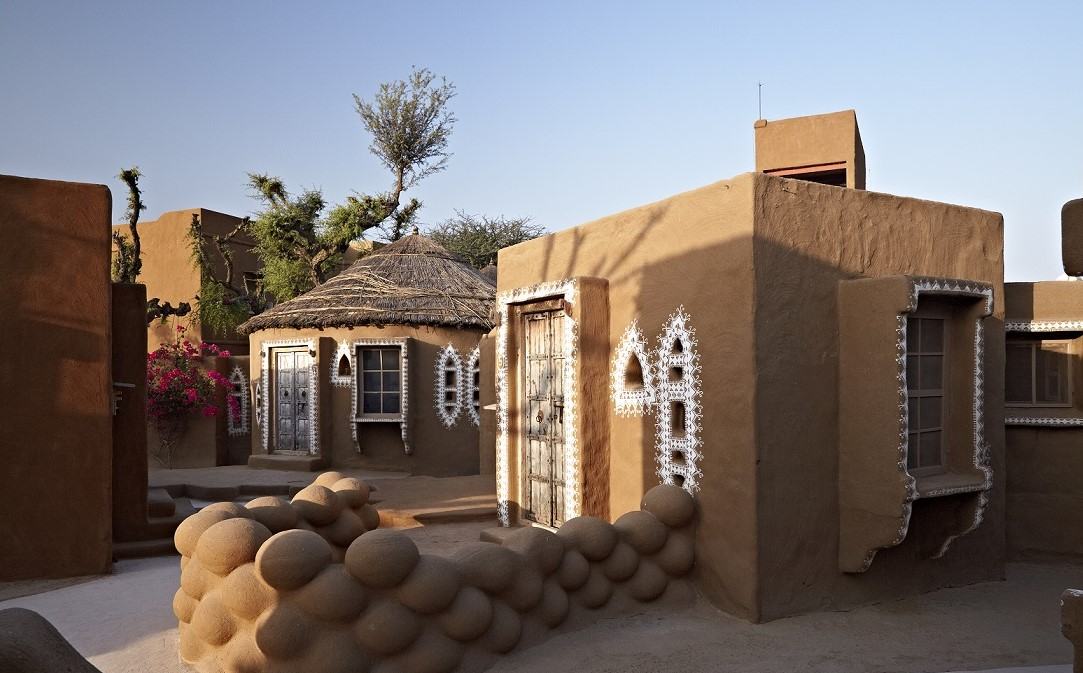
\includegraphics[angle=0,width=1.0\textwidth]{img/dc-01}
  \caption{The Desert Camp -- A poem in mud}
  \label{fig:dc-01} 
\end{figure}

\noindent Social interaction in rural area is the core concept of this design. Everyone in an Indian village knows what everyone else is doing, encouraging curiosity and inquisitiveness as a way to create a sense of community bonding. This consideration one can easily notice through this design.

% section dcm_concept (end)

\subsection{Site conditions} % (fold)
\label{sub:dcm_sitecond}

The site is on a large sand dune that rises upward into a hillock on which rests a shrine dedicated to Gugaji --- the saint of the serpents. It is understood that there was once an old settlement on this site with a flowing river through it. In the words of the architect, ``The fact that the site was associated with ancient times was most exciting, and therefore it was the main inspiration and guiding force in the evolution of its design --- the plan and spatial organisations as well as the materials and the methods of construction.''

% subsection dcm_sitecond (end)

\subsection{Planning and circulation} % (fold)
\label{sub:dcm_planning}

The huts form a cluster of eight --- two are meant to represent farmers, three of weavers and three of potters. They are neither arranged in a row not do they share common walls. Each one is a separate unit and yet part of the group. Social interaction in our rural areas being what it is, spaces have been provided where the fabric of everyday interactions is woven.

The suites are designed to be accommodated in a cluster of buildings, which constitute one house, and are grouped around a courtyard. The clusters then come together to form the main village street. The spatial sequence, plans, and architectural elements of the clusters are based upon the house forms of the weaver, the potter, and the farmer. But the plans are not mere transpositions. The traditional morphology has been extended to accommodate a new complexity, because a hotel room cannot just be a loom room for five star rates.

No two huts are similar. Though what they all have in common are the furnished features of comfort --- lights, fans, tiled bathrooms with western-style water closets and showers with running hot and cold water, which seem a bit incongruous in these surroundings, but a necessity for the modern traveller.

A chakki, a grinding stone, etc., are embedded in the platforms and steps outside huts to indicate how people sit and chat while going about their everyday chores, or how neighbours walking past stop to exchange pleasantries.

Slightly away from the huts is the dining and kitchen units in conjunction with the reception and lounge. The latter leads through the lawns to the swimming and wading pools.

\begin{figure}[H]
  \centering
  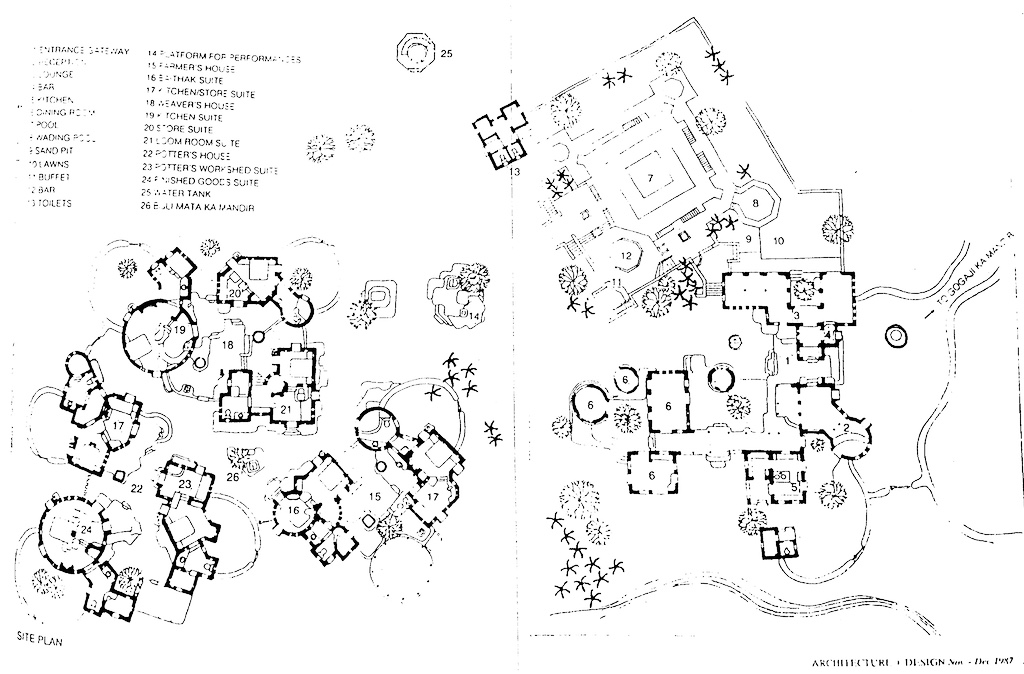
\includegraphics[angle=90,width=1.0\textwidth]{img/dc-02}
  \caption{Plan view of The Desert Camp}
  \label{fig:dc-02} 
\end{figure}

\begin{figure}[H]
  \centering
  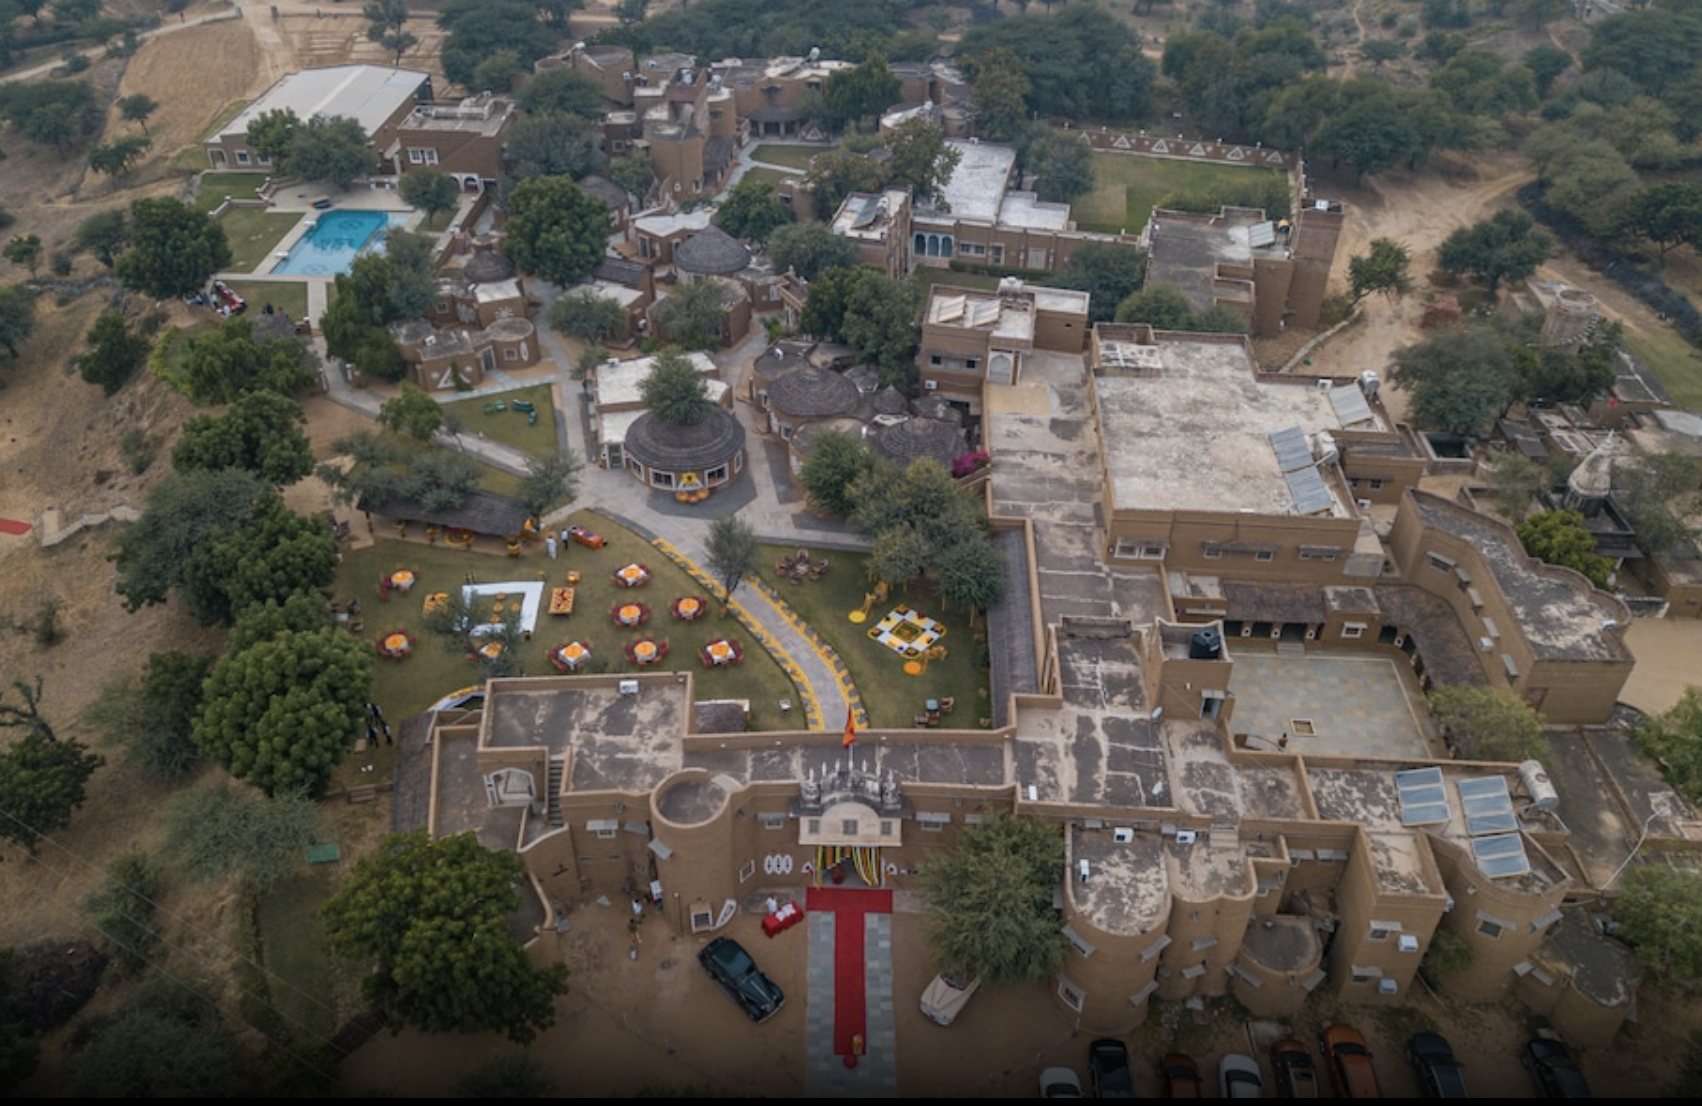
\includegraphics[angle=90,width=1.0\textwidth]{img/dc-av}
  \caption{Aerial view of The Desert Camp}
  \label{fig:dc-av} 
\end{figure}

\begin{figure}[H]
  \centering
  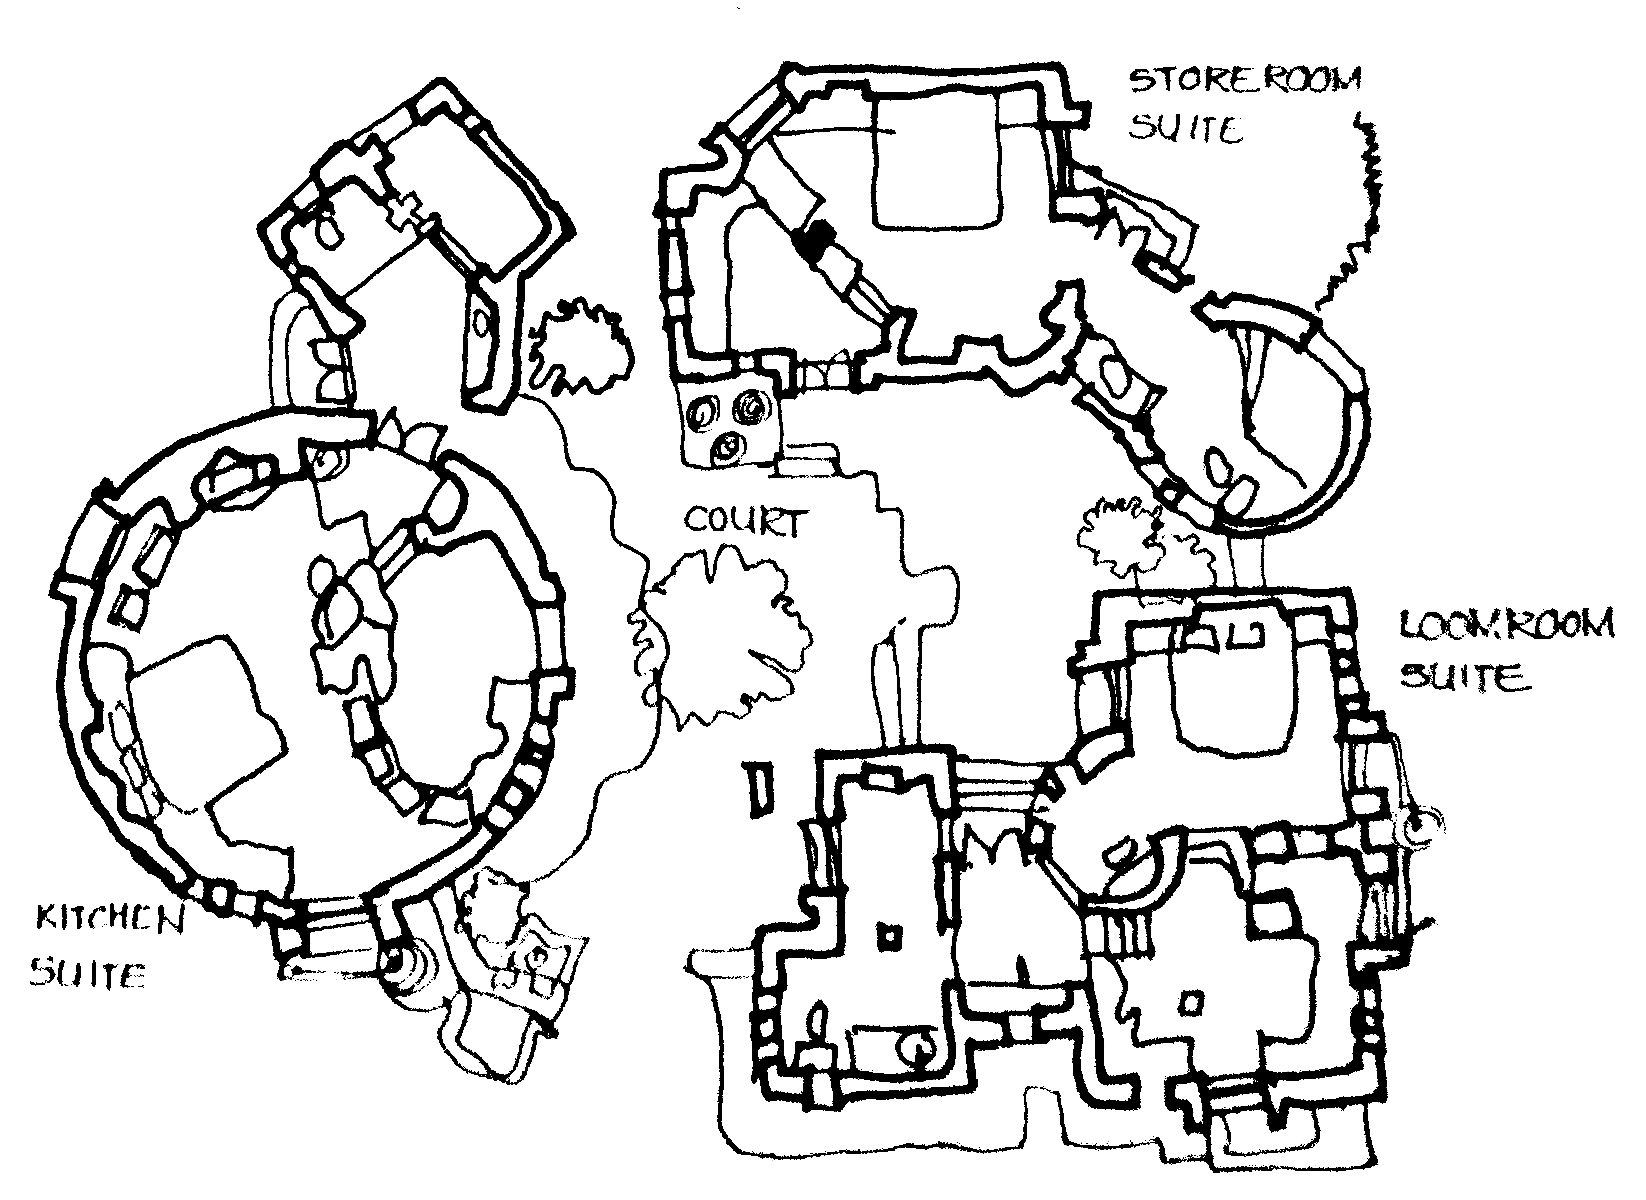
\includegraphics[angle=0,width=1.0\textwidth]{img/dc-03}
  \caption{Cluster of weavers' huts}
  \label{fig:dc-03} 
\end{figure}

\begin{figure}[H]
  \centering
  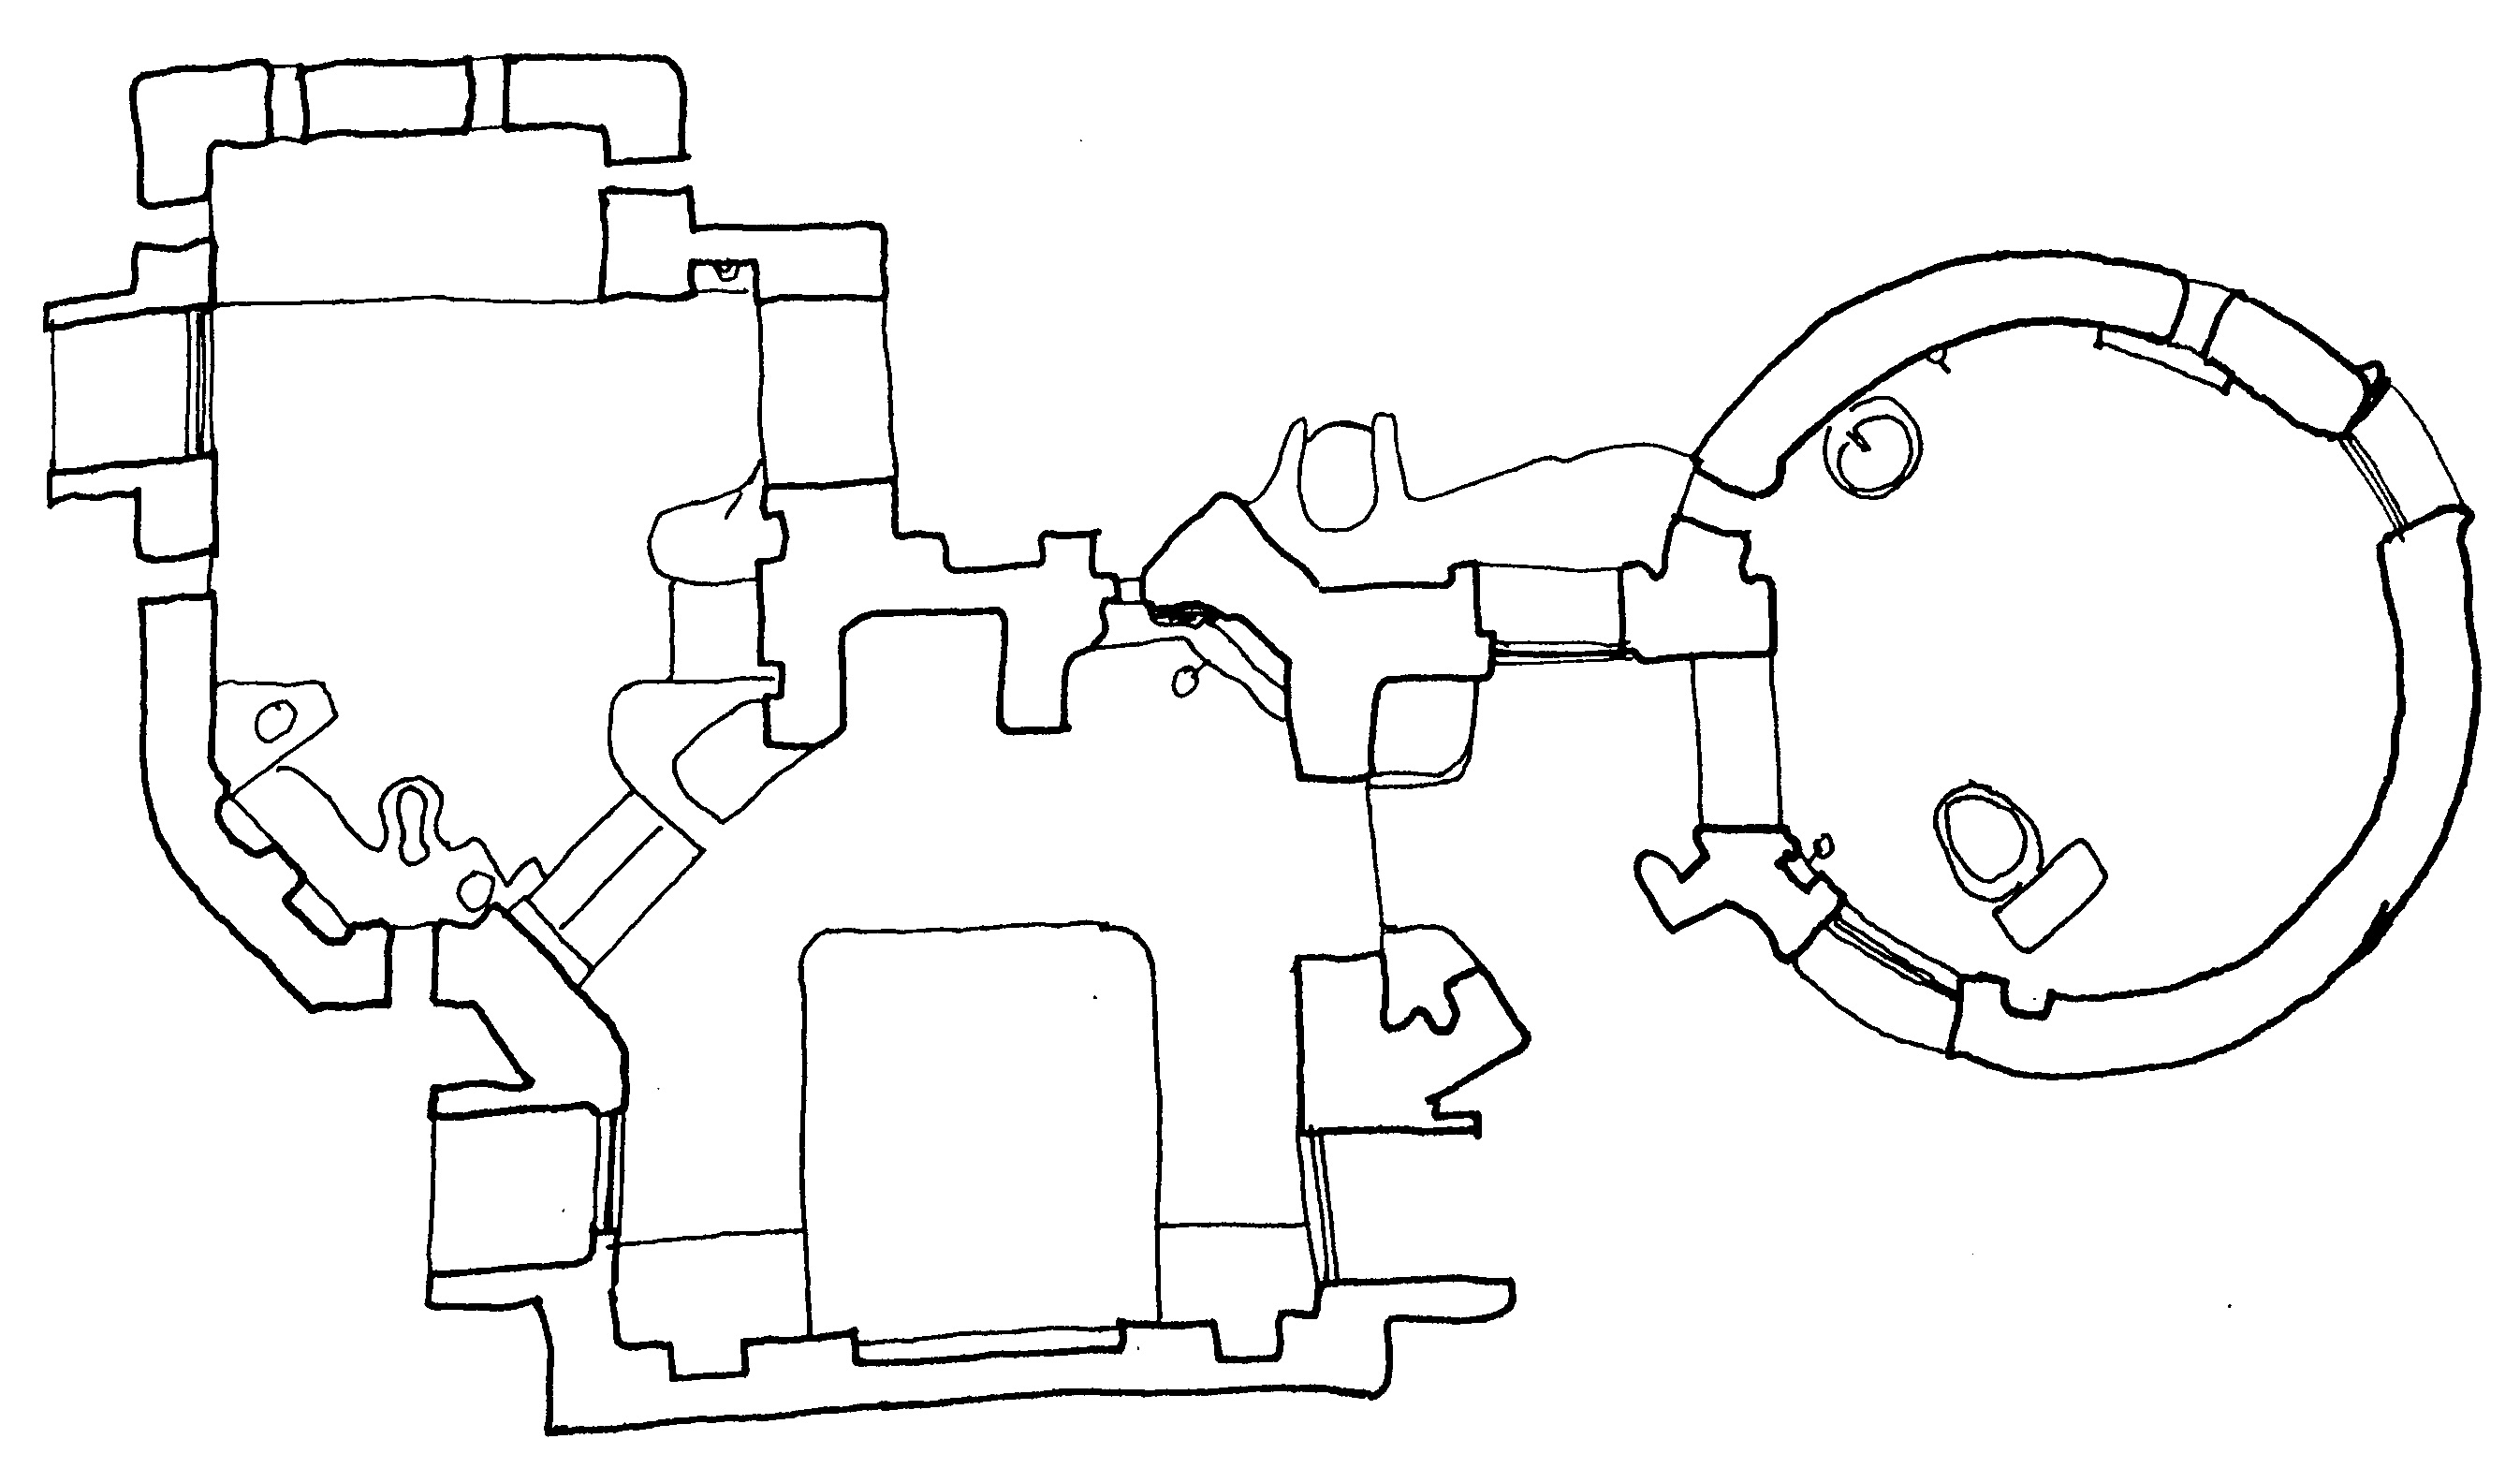
\includegraphics[angle=0,width=1.0\textwidth]{img/dc-04}
  \caption{Farmer's hut}
  \label{fig:dc-04} 
\end{figure}

\begin{figure}[H]
  \centering
  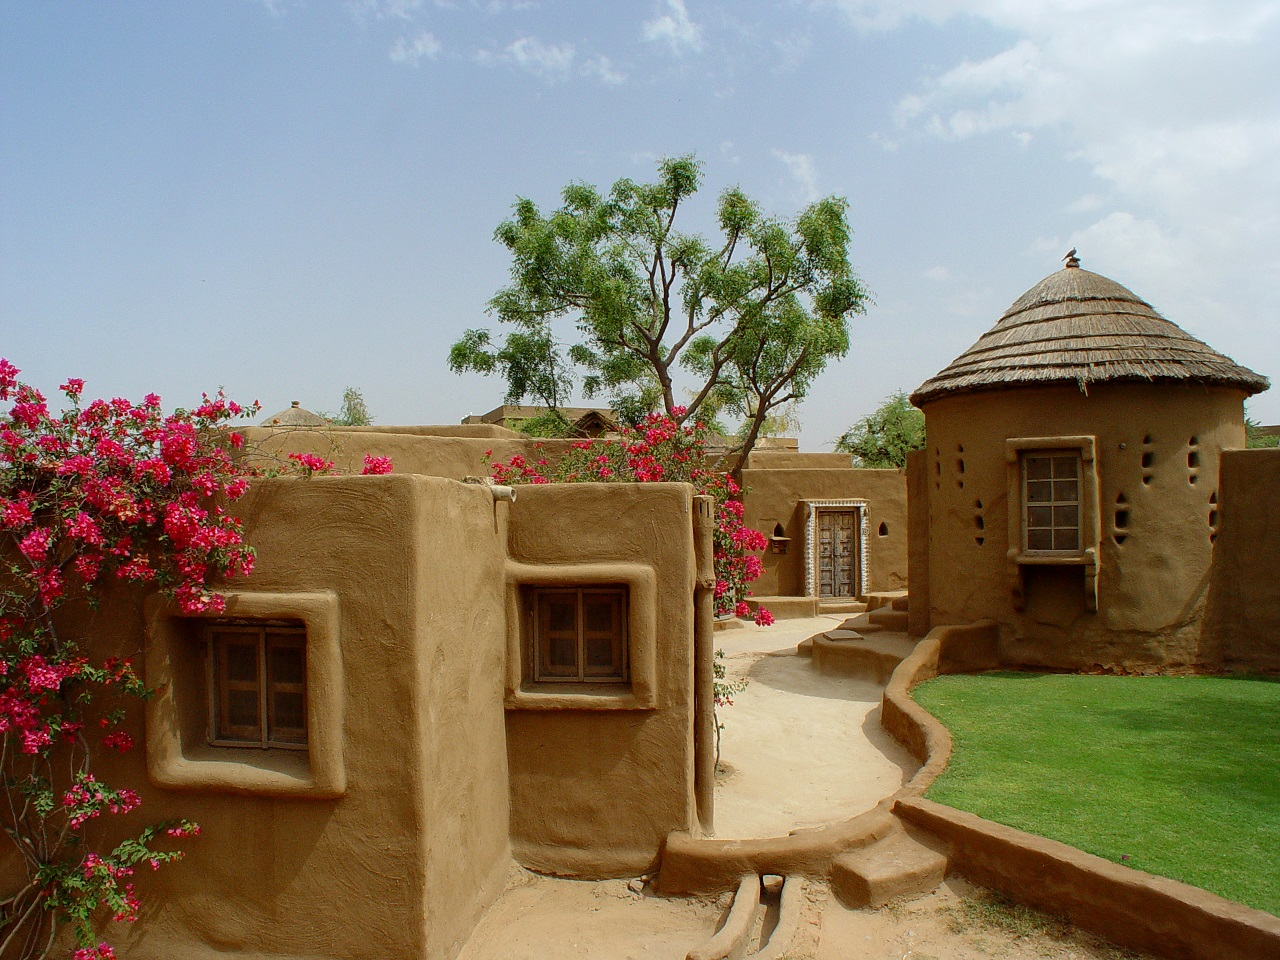
\includegraphics[angle=0,width=1.0\textwidth]{img/dc-fh}
  \caption{An overview of farmer's hut}
  \label{fig:dc-wh} 
\end{figure}

% subsection dcm_planning (end)

\subsection{Construction techniques used} % (fold)
\label{sub:dcm_ctu}

The project employed local masons, carpenters, lathe workers, stone craftsmen, and most importantly all the skills of rural women, woman's touch to the setting, in both the execution and the finish.

While justifying the use of mud for the entire complex, the architect says, ``I work with these materials because they are beautiful and powerful. When you work with mud and hand-plaster the walls, it is like forming an external skin; it is as every bit of the building embodies the human spirit, the cyclic core of the building being a part of the act of living.''

The architects were already aware of the architectural traditions of rural areas of Shekhawati, having worked with some migrants from the area. The project involved rekindling images and memories of a home that they carried, and translating them into series of sketches.

Most materials used in the work are the sun-dried bricks, thatch, stone for foundations, sills, lintels, brackets, roofing slabs, and most of the built-in structure. These were made available from nearby places within the 30km radius. The wooden lathe workers made pegs and other small fixtures, which the local carpenters put them together and carved them. Local masons built structures, and the women from nearby villages finished the walls with mouldings, relief work, embedded mirror work, and also mould in mud elements such as tools, platforms, grain bins (obri) and stones (khota), etc.

% [Image here: Detail of thatched roof]

The floors are plastered with cow-dung. Some roofs are thatched while others have unpolished stone slabs. The work on the thatched roof is interesting with their perfect concentrated circles formed by bamboo strips holding straws together, they seem meticulously crafted. Not a piece out of line, each fitting perfectly in its groove.

The building is built on brick foundations, as are the walls, sleeping platforms, ledges, etc., and are plastered with cow-dung. Outside, the walls and the windows are decorated with motifs painted in white.

\begin{figure}[H]
  \centering
  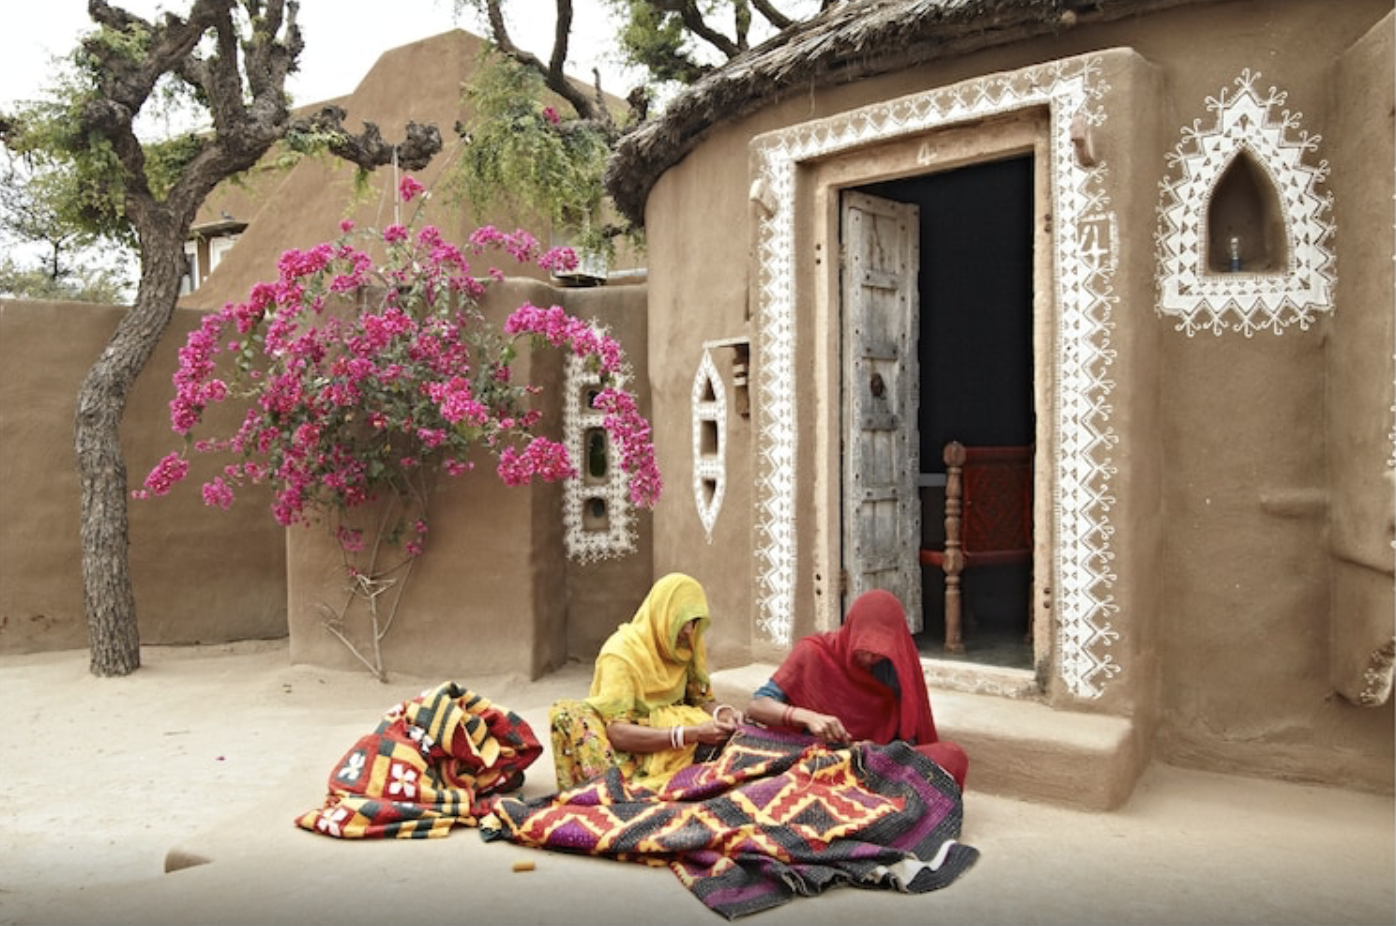
\includegraphics[angle=0,width=1.0\textwidth]{img/dc-05}
  \caption{Detail of painted walls and window borders. Artisan women working in the foreground}
  \label{fig:dc-05} 
\end{figure}

\noindent It can be noted here that the traditional morphology has been extended to accommodate a new complexity, because a hotel suite cannot just be a loom room, dressing room, and a water closet. A novel idea in the huts are the mirrors embedded in the walls with niches on sides. With the stool below, they become natural dressing tables.

\begin{figure}[H]
  \centering
  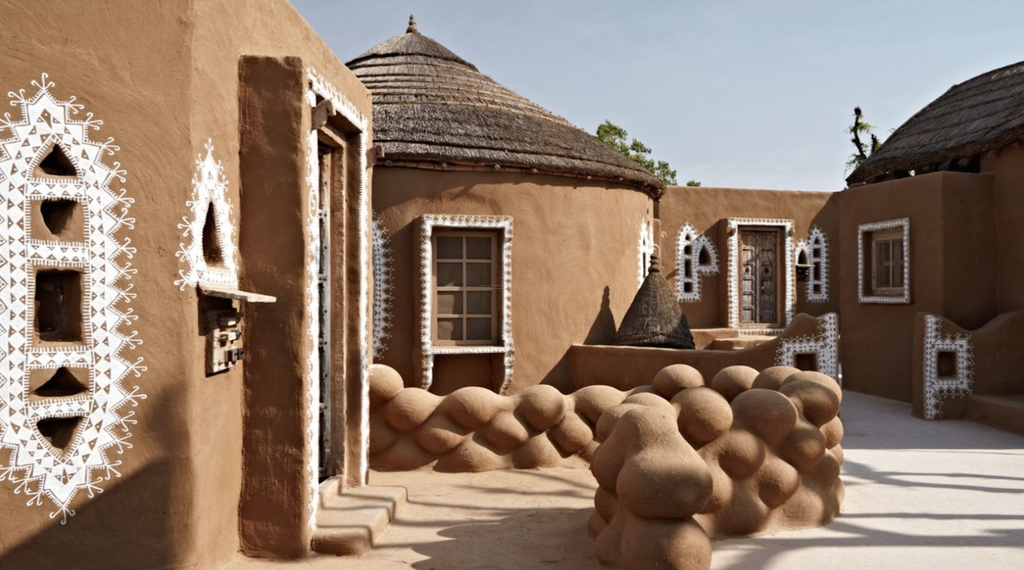
\includegraphics[angle=0,width=1.0\textwidth]{img/dc-06}
  \caption{Peculiar way of construction of compound walls}
  \label{fig:dc-06} 
\end{figure}

\begin{figure}[H]
  \centering
  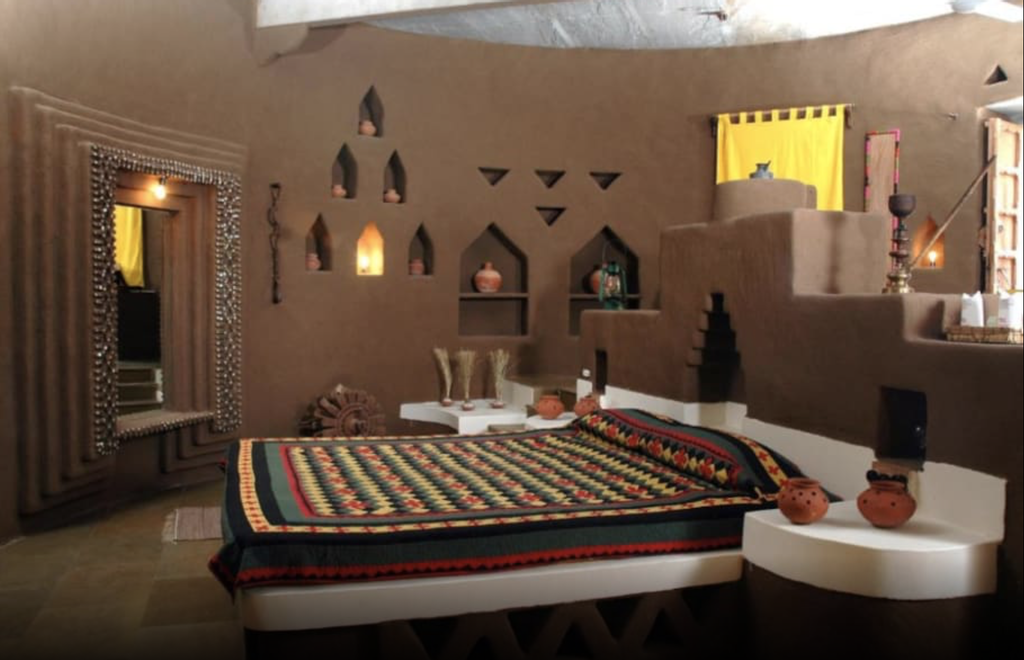
\includegraphics[angle=0,width=1.0\textwidth]{img/dc-07}
  \caption{An artistic arrangement of the built-in furniture including the dressing table}
  \label{fig:dc-07} 
\end{figure}

\noindent Huts are furnished with simple cotton fabrics, and yet the patchwork quilts and bed covers, made by the villagers are strikingly colourful. Over sleeping platforms, foam mattresses have been used for comfort in lieu of a bed.

Each hut is decorated with the implants and tools required by a potter, a weaver or a farmer. Bright cloth edged with silver gota have been draped above some beds, while the niches in walls hold pottery and other wares as decorative, as well as utility items.

Thus, at this place an urban dweller can truly enjoy a taste of rural living, close to the earth and under the stars. The designer has paid due attention to details to ensure that the tourist would face no discomfort.

% subsection dcm_ctu (end)

% section dcm (end)